\documentclass[a4paper, 11pt, titlepage]{article}
\usepackage{fancyhdr}
\usepackage{graphicx}
\usepackage{imakeidx}
\usepackage{makeidx}
\usepackage{mathtools}
\usepackage[spanish]{babel}
\usepackage{eurosym}
\usepackage{hyperref}
\usepackage{amssymb}
\usepackage{listings}
\usepackage{xcolor}

\setcounter{secnumdepth}{5}
\setcounter{tocdepth}{5}

\title{Criptografía}
\author{Francisco Javier Balón Aguilar}

\begin{document}

\maketitle
\renewcommand{\contentsname}{Índice}
\tableofcontents
\newpage

\section{Criptografía práctica sobre entorno GNU/Linux}

    \subsection{GnuPG (gpg)}
        
    GnuPG, a veces denominado simplemente gpg (siglas de GNU Privacy Guard) es un derivado libre
    de PGP. Su utilidad es la de cifrar y firmar digitalmente. gpg soporta tanto cifrado simétrico 
    como cifrado asimétrico.

    gpg tiene un repositorio de claves, llamado \textbf{anillo de claves} 
    donde almacena todas las claves que tenemos en nuestro sistema; sean privadas o públicas.

    Los \textbf{servidores de claves} ayudan a difundir las claves públicas 
    de forma que podamos compartirlas fácilmente para que otros usuarios puedan utilizarlas y
    cifrar con ellas.

    \subsubsection{Cifrado simétrico}

        El cifrado simétrico es sencillo; se utiliza la misma clave para cifrar y para descifrar.
        Es rápido de procesar y sencillo de usar, como contraposición, tiene la desventaja de la 
        comunicación de la clave\footnote{
            Tanto $A$ como $B$ deben conocer la misma clave. Por lo que si $A$ cifra un texto con
            la clave $123$, debe en algún momento comunicarla a $B$ para que éste pueda descifrarla.
            En esta comunicación encontramos un posible vector de ataque para obtener la clave.
        }.

        El uso de gpg con cifrado simétrico es muy sencillo. Simplemente llamamos a un texto sin cifrar
        con el parámetro $-c$ (crypt, cifrar) lo que generará un archivo en formato \textit{.gpg} cifrado
        por defecto con el algoritmo AES con la clave proporcionada (véase figuras \ref{crypt01} y 
        \ref{crypt02}).

        \begin{figure}[htp]
            \centering
            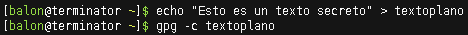
\includegraphics[width=0.8\textwidth]{resources/crypt01.png}
            \caption{Cifrado simétrico de archivo de texto.}
            \label{crypt01}
        \end{figure}

        \begin{figure}[htp]
            \centering
            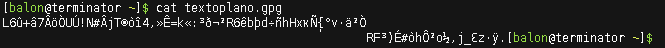
\includegraphics[width=0.8\textwidth]{resources/crypt02.png}
            \caption{Texto cifrado gpg.}
            \label{crypt02}
        \end{figure}

        Para descifrarlo, simplemente hay que pasarle a gpg el parámetro $-d$ (decrypt, descifrar) y el archivo 
        previamente cifrado (véase figura \ref{decrypt01}).

        \begin{figure}[htp]
            \centering
            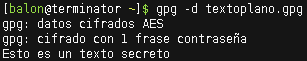
\includegraphics[width=0.5\textwidth]{resources/decrypt01.png}
            \caption{Texto descifrado con gpg con algoritmo simétrico AES.}
            \label{decrypt01}
        \end{figure}

    \subsubsection{Cifrado asimétrico}
        
        % TODO: genbeta.com/desarrollo/manual-de-gpg-cifra-y-envia-datos-de-forma-segura

        \subsubsection{Generación de par de claves}

        \subsubsection{Exportación e importación de claves}

        \subsubsection{Cifrado con clave pública}

        \subsubsection{Descifrado con clave privada}

    \subsubsection{Firma digital de archivos}

        \paragraph{Verificación y descifrado de archivos firmados}

    \subsubsection{Confiabilidad de claves}

    \subsection{SSH}

    % TODO: solvetic.com/tutoriales/article/1815-el-manual-del-secure-shell/
    \subsubsection{El cliente SSH}
    \subsubsection{El servidor SSH}
    \subsubsection{Securización de SSH}
    \subsubsection{Autenticación mediante intercambio de claves asimétricas (RSA)}

        Como ya hemos visto, una conexión común usando el protocolo SSH es de por sí 
        segura; al menos más segura que una conexión no cifrada como telnet, pero presenta,
        \textit{grosso modo} dos inconvenientes:

        \begin{enumerate}
            \item La contraseña, aún yendo cifrada, viaja por la red siempre que nos autenticamos.
            Esto puede ser peligroso en el caso que haya alguien capturando el tráfico de nuestra 
            red (\textit{sniffing}) y fuese capaz de descifrar nuestra clave (mediante ataques por 
            fuerza bruta o diccionario, utilizando alguna vulnerabilidad conocida, etc. Es muy 
            complicado, pero no imposible).
            \item En el caso de manejar numerosos servidores y conexiones SSH puede ser muy tedioso 
            tener que estar recordando contraseñas, almacenandolas, etc. Este método agregaría un plus 
            de comodidad y escalabilidad a las conexiones.
        \end{enumerate}

        La implementación del algoritmo RSA presenta solución a estos problemas. Su funcionamiento
        es:

        \begin{enumerate}
            \item El cliente envía información sobre su clave pública al servidor.
            \item El servidor busca en su base de datos la clave pública del cliente y, cuando la encuentra,
            envía al cliente un \textit{challenge} (desafío), que contiene un número aleatorio generado y 
            cifrado por éste utilizando la clave pública del cliente.
            \item El cliente recibe el paquete cifrado y usa su clave privada para descifrarlo y devolvérselo 
            al servidor.
            \item El servidor comprueba que el número devuelto es el que mandó cifrado, en caso afirmativo, el 
            usuario se ha autenticado y se le permite la sesión de shell.
        \end{enumerate}

        Como observamos, en ningún momento se envían claves por Internet (más que el envío 
        de la clave pública al servidor en el primer contacto, para que éste la conozca). Por 
        supuesto si alguien accede a nuestro equipo y nos roba la clave privada podría autenticarse 
        como nosotros y suplantar nuestra identidad criptográfica. Por esta razón es necesario 
        proteger las distintas formas de acceso, desde cifrado de particiones a configuración 
        estricta de permisos. 
        
        También es posible asignar un cifrado simétrico sobre las claves asimétricas, dando una 
        capa extra de seguridad a cambio de tener que introducir una clave cada vez que la usemos.
        
        \paragraph{Configuración en servidor sshd} La configuración en el servidor es sencilla,
        simplemente deberemos acceder a éste y habilitar la autorización a través de RSA. Esto lo haremos 
        en su archivo de configuración añadiendo o descomentando las líneas:

        \begin{lstlisting}[language=bash]
    # /etc/ssh/sshd_config
    RSAAuthentication yes
    PubkeyAuthentication yes
    AuthorizedKeysFile %h/.ssh/authorized_keys\end{lstlisting}

        Véase la última línea, donde añadimos el fichero que almacenará las claves públicas 
        de los clientes reconocidos. Si no existiera este directorio y/o fichero deberemos crearlo.

        \paragraph{Generación de par de claves en cliente} En el cliente crearemos el par de claves 
        (pública y privada) en algoritmo RSA. Para ello simplemente usaremos 

        \begin{lstlisting}[language=bash,basicstyle=\scriptsize]
    $ ssh-keygen -t rsa
    Generating public/private rsa key pair.
    Enter file in which to save the key (/home/balon/.ssh/id_rsa): 
    /home/balon/.ssh/rsa
    Enter passphrase (empty for no passphrase): 
    Enter same passphrase again: 
    Your identification has been saved in /home/balon/.ssh/rsa
    Your public key has been saved in /home/balon/.ssh/rsa.pub
    The key fingerprint is:
    SHA256:aVgQfYrakZnFhaw4Gcl0bHqrJj7QtR3dXm332wx9qdE balon@terminator
    The key's randomart image is:
    +---[RSA 3072]----+
    |   o.o+= o.      |
    |    +.o.* .      |
    |     * O.+   .   |
    |    * Xoo.. . o .|
    | . . B.+S. . ..oo|
    |. . o +.  .  ..E+|
    | .   .        oo+|
    |  o o        . .o|
    | ..+             |
    +----[SHA256]-----+\end{lstlisting}

        A continuación debemos configurar el \textit{ssh-agent} para añadirle nuestra 
        clave privada emparejada con la pública que enviaremos al servidor, de forma que,
        ejecutándose junto a la sesión, éste esté vinculado a ella directamente.

        \begin{lstlisting}[language=bash,basicstyle=\small]
    $ eval $(ssh-agent -s)
    Agent pid 15081
    $ ssh-add ~/.ssh/rsa
    Identity added: /home/balon/.ssh/rsa 
    (/home/balon/.ssh/rsa) \end{lstlisting}

        Esto además evitará que tengamos que poner nuestra contraseña simétrica 
        para descifrar la clave privada, en caso que hayamos configurado una, ya que la 
        el agente SSH de la sesión se encargará de descifrarlo, ganando comodidad y velocidad.

        \paragraph{Intercambio de clave pública entre cliente y servidor} Una vez hemos 
        generado el par de claves es momento de la clave pública generada al servidor 
        (ésta suele tener la terminación \textit{.pub}). La forma de enviarla podrá ser 
        la deseada por el usuario, en este caso utilizaremos el protocolo SCP (véase 
        sección \ref{scp} para más información). Véase que es el único momento donde se 
        envía la clave.
        
        \begin{lstlisting}[language=bash]
    $ scp ~/.ssh/rsa.pub root@server:/tmp
    root@server's password:
    rsa.pub \end{lstlisting}

        En el servidor deberemos pues añadir la clave recibida al fichero \textit{authorized\_keys}
        que configuramos previamente.
        
        \begin{lstlisting}[language=bash,basicstyle=\scriptsize]
    $ cat /tmp/rsa.pub
    ssh-rsa AAAAB3NzaC1yc2EAAAADAQABAAABgQCoaiQqlc0hhqdVsh52sB/ui
    ISb1pRU/6DVWqyvpCYWQOd8PGNGjuFwYeOnTQ1mZYppuNoXmQxzKXJXGK4ke/
    4HcgRHj9l2zZL0LBacnU1NEszqVYUgpI4+1qbyMi0LQZTpKedGULFcSVa1QDt
    SWTLeQIYTK7dphN4wo7cer9EFkfj5Z1ZNWSjC4blTFTGD2L03aSUklek+BHkk
    FFGYmVKw/+VD7aOA+Imsb/qHp1eUhEKcHSlWPfDS6qf+GwJoB72v4TMCH1At1
    fM2LP8o/eRF31fZdRJGOHL+MzfXR0RqS1SLfr/1g6NRohmu1BFFdQQxisovPf
    h1iOBs4apqQjRl6P6qQziwSVShkkzDW0xOnIflWwbYjo/w1SFN5YzwDaOV3QK
    VYEeHQGm2mdwPGqPxyeyTaCZqf5Ca2k/Gv53BlRCUb3ATpXTbN6HzIliOUtFm
    idUAYQwYM0n7VMpL7NW+/1ap6UthX/ep/CjcxGqYZc4+iTSSSict9caCSGSY+
    Ec= balon@terminator
    $ cat /tmp/rsa.pub >> .ssh/authorized_keys
    $ cat .ssh/authorized_keys
    ssh-rsa AAAAB3NzaC1yc2EAAAADAQABAAABgQCoaiQqlc0hhqdVsh52sB/ui
    ISb1pRU/6DVWqyvpCYWQOd8PGNGjuFwYeOnTQ1mZYppuNoXmQxzKXJXGK4ke/
    4HcgRHj9l2zZL0LBacnU1NEszqVYUgpI4+1qbyMi0LQZTpKedGULFcSVa1QDt
    SWTLeQIYTK7dphN4wo7cer9EFkfj5Z1ZNWSjC4blTFTGD2L03aSUklek+BHkk
    FFGYmVKw/+VD7aOA+Imsb/qHp1eUhEKcHSlWPfDS6qf+GwJoB72v4TMCH1At1
    fM2LP8o/eRF31fZdRJGOHL+MzfXR0RqS1SLfr/1g6NRohmu1BFFdQQxisovPf
    h1iOBs4apqQjRl6P6qQziwSVShkkzDW0xOnIflWwbYjo/w1SFN5YzwDaOV3QK
    VYEeHQGm2mdwPGqPxyeyTaCZqf5Ca2k/Gv53BlRCUb3ATpXTbN6HzIliOUtFm
    idUAYQwYM0n7VMpL7NW+/1ap6UthX/ep/CjcxGqYZc4+iTSSSict9caCSGSY+
    Ec= balon@terminator\end{lstlisting}
        
        Una vez finalizado, podremos realizar comunicaciones SSH entre el cliente y 
        el servidor directamente usando las claves RSA, ganando seguridad y comodidad 
        en las comunicaciones.

    \subsubsection{Exportación e importación de claves}
    \subsubsection{Generación de \textit{passphrase} y asociación con \textit{ssh-agent}}
    \subsubsection{SCP} \label{scp}
    \subsubsection{SFTP}

    % TODO: profesionalreview.com/2016/09/10/como-encriptar-datos-en-linux-ubuntu-linux-mint
    \subsection{VeraCrypt}
    \subsection{Files}
    \subsection{LUKS}
    \subsection{eCryptfs}
    \subsection{AESCrypt}

\section{Esteganografía práctica sobre el entorno GNU/Linux}

    \subsection{Steghide}

    % TODO: 2daygeek.com/easy-way-hide-information-inside-image-and-sound-objects

\end{document}